\documentclass{beamer}
\usepackage{color}
\usepackage{amsfonts}
\usepackage[MeX]{polski}
\usepackage[utf8]{inputenc}
\usepackage[tableposition=top]{caption}
\usepackage{algorithmic}
\usepackage{graphicx}
\usepackage{enumerate}
\usepackage{multirow}
\usepackage{amsmath} %pakiet matematyczny
\usepackage{amssymb} %pakiet dodatkowych symboli
\usepackage{xcolor}
\usepackage{booktabs}
\usepackage{sidecap}
\usepackage{wrapfig}
\usepackage{caption}
\begin{document}
\begin{frame}
\frametitle{Tygrys azjatycki}
 Tygrys azjatycki, tygrys  – gatunek dużego, drapieżnego ssaka łożyskowego z rodziny kotowatych, największy z żyjących współcześnieczterech wielkich, ryczących kotów z rodzaju Pantheraświęte.
\end{frame}

\begin{frame}
\begin{figure}

\centering
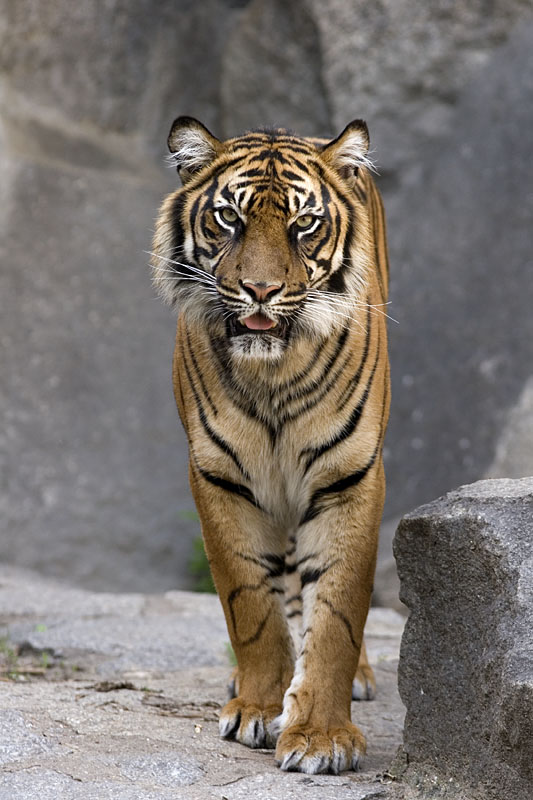
\includegraphics[width=0.5\textwidth]{tigris.jpg}
\end{figure}
\end{frame}
 \begin{frame}
 \frametitle{Pochodzenie tygrysa}
 Filogeneza tygrysów nie została jednoznacznie wyjaśniona. Współczesna wiedza o pochodzeniu tych drapieżników opiera się na niewielkiej ilości materiału kopalnego. Wszystkie żyjące współcześnie duże koty zaliczane są do podrodziny Pantheriinae. 
 \end{frame}
 % itd ...
\begin{frame}
 \frametitle{Umaszczenie}
 \begin{figure}
\caption{Białe tygrysy}
\centering
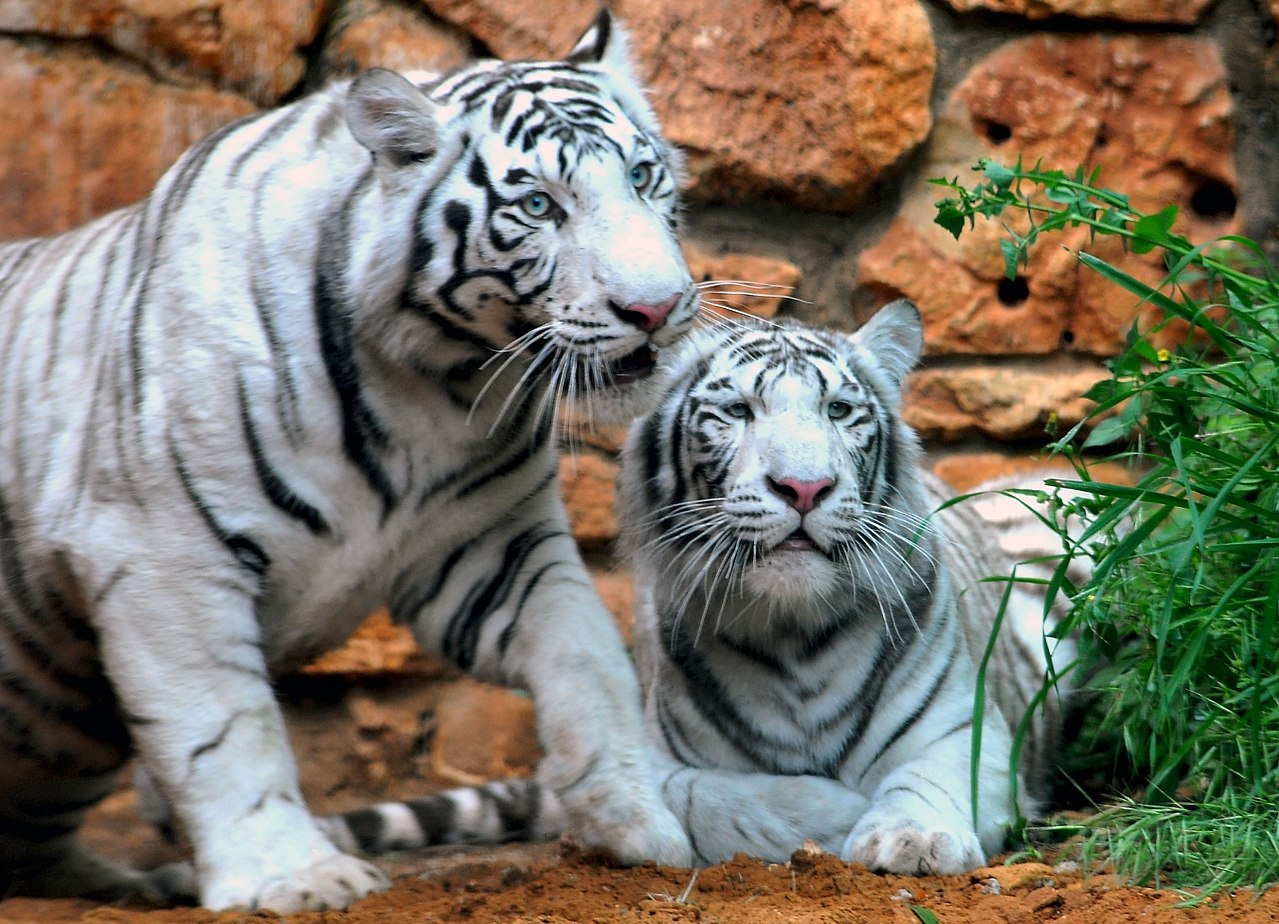
\includegraphics[width=0.5\textwidth]{White_Tigers.jpg}
\end{figure}
\end{frame}

\begin{frame}
 \begin{figure}
\caption{Czarne tygrysy}
\centering
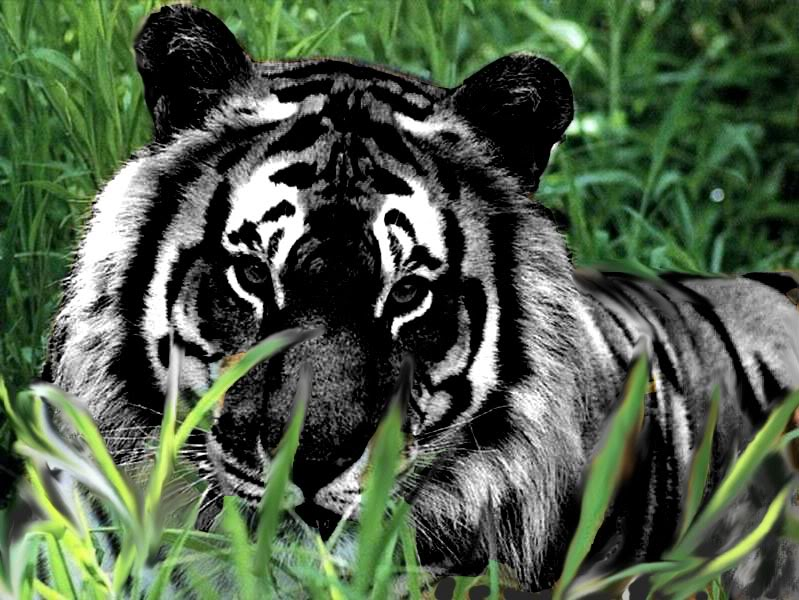
\includegraphics[width=0.5\textwidth]{Black_Tiger.jpg}
\end{figure}
\end{frame}

\begin{frame}
 \begin{figure}
\caption{Niebieskie tygrysy}
\centering
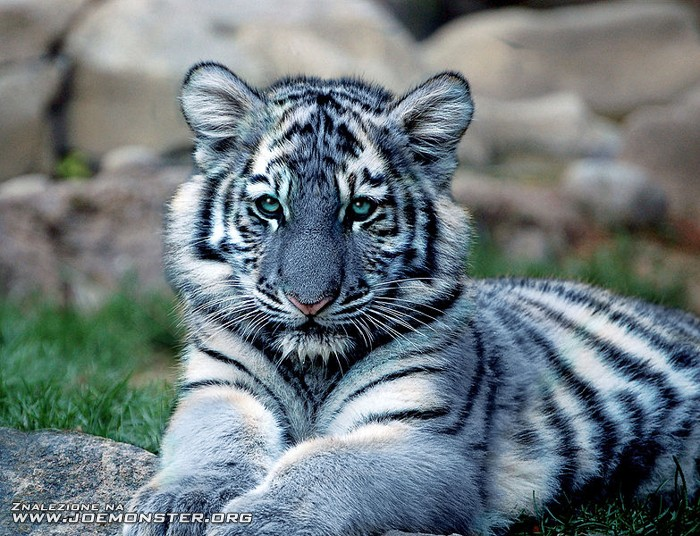
\includegraphics[width=0.5\textwidth]{niebieski_tygrys.jpg}
\end{figure}
\end{frame}

\begin{frame}
 \begin{figure}
\caption{Golden Tabby}
\centering
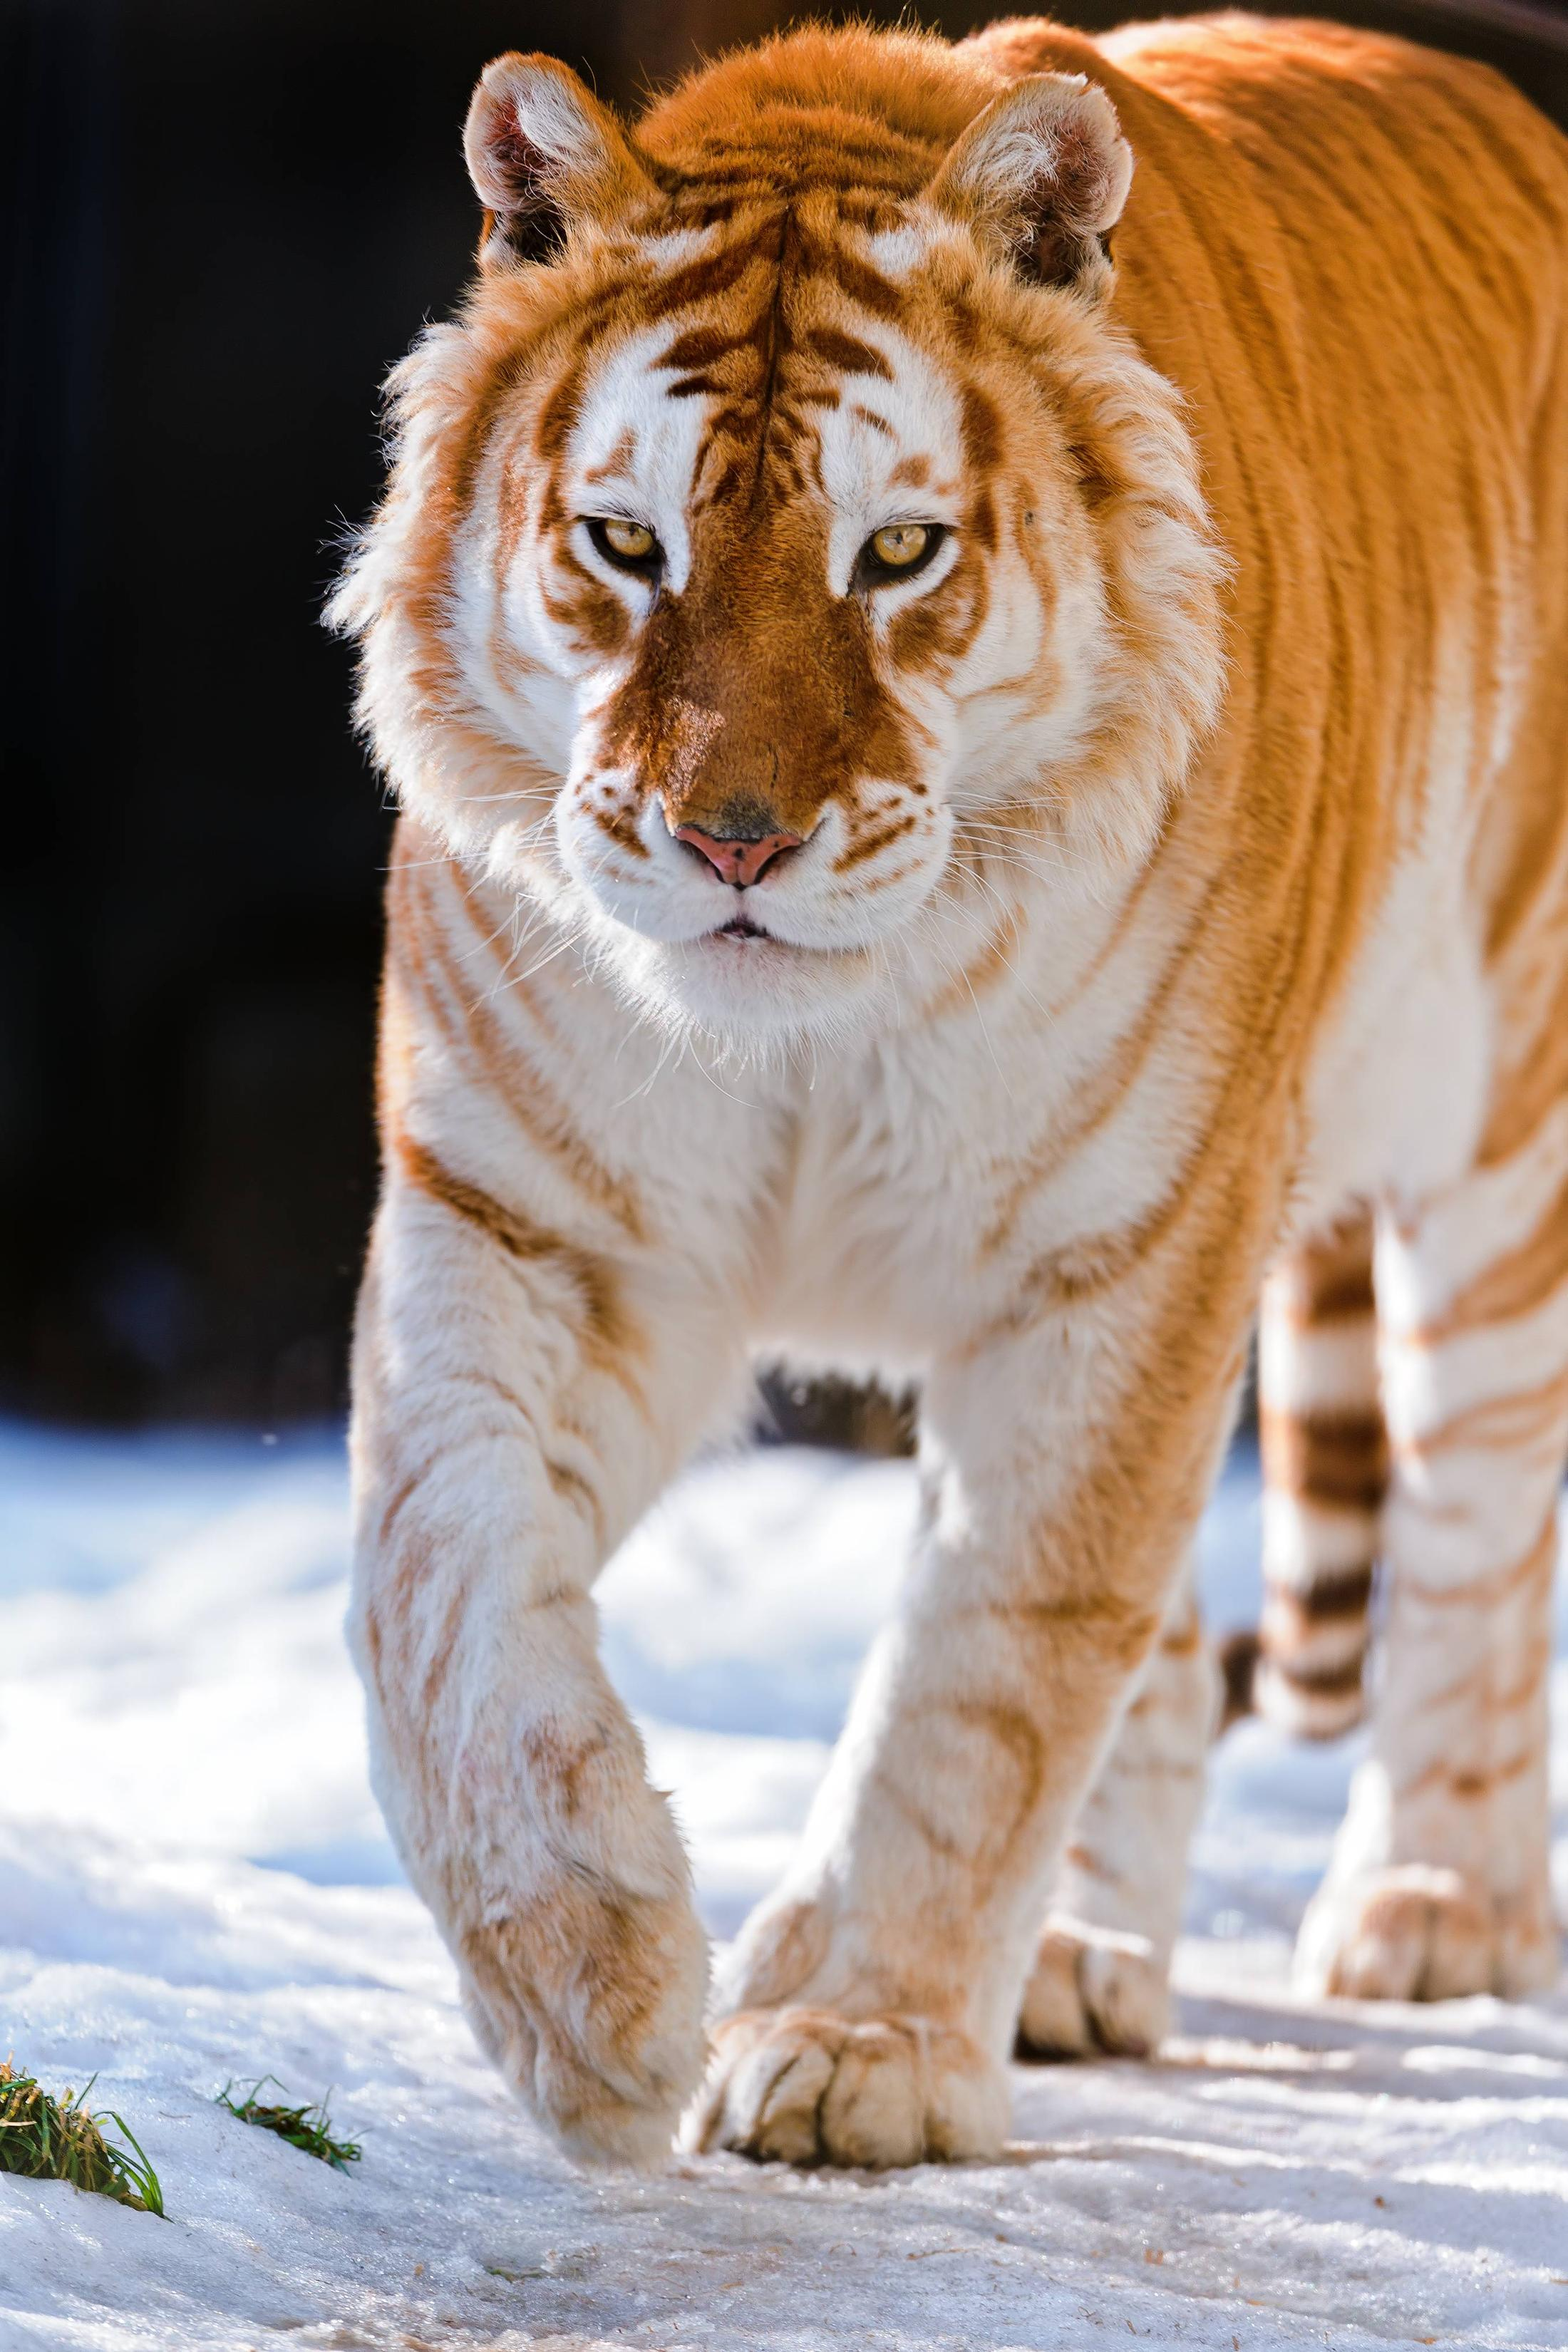
\includegraphics[width=0.5\textwidth]{cJUlOim.jpg}
\end{figure}
\end{frame}

\AtBeginSection[]
{
\begin{frame}
\frametitle{Spis treści}
\tableofcontents[currentsection]
}
 
 
\end{document}